\chapter{Nt32-IA32持续集成测试系统的设计与实现}
\label{cha:intro}

\section{Nt32-IA32的背景介绍}
	
	Nt32是以VS2013提供的函数库为基础开发的一种平台的UEFI BIOS,其编译生成的Nt32模拟器可以用于仿真模拟UEFI BIOS环境。因此可以利用该平台模拟出整个对UEFI BIOS分析测试的过程。
	
	在本章中,我们以Nt32平台为例,说明在该种平台下的持续集成测试系统的搭建。最终的完成目标是:在IA-32架构的(特定的CPU架构)Nt32平台上,实现对该种架构的UEFI BIOS平台持续集成测试系统的搭建,并且应用到Nt32-IA32的实际开发项目中去。

\section{Nt32-IA32持续集成测试系统的设计方案}
	\subsection{Nt32-IA32持续集成测试系统的环境组成}
		
		Nt32-IA32持续集成测试系统的环境组成如图~\ref{fig:Nt32-IA32持续集成测试系统的环境组成}所示:
		
		\begin{figure}[H] % use float package if you want it here
			\centering
			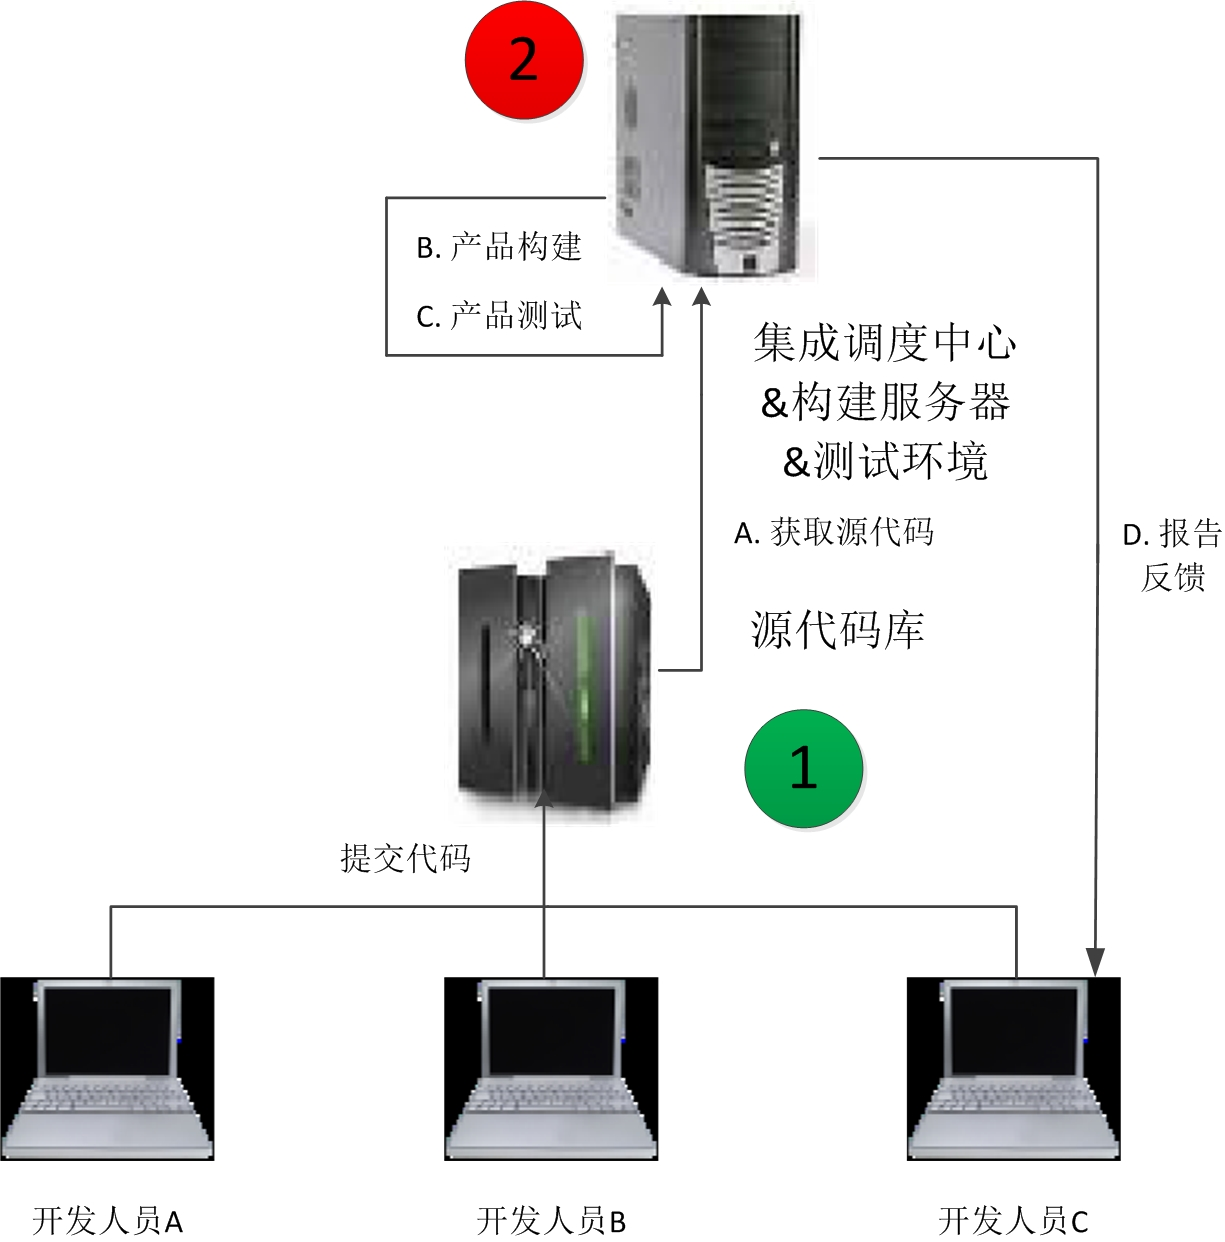
\includegraphics[height=10cm]{chart5/Nt32-IA32持续集成测试系统的环境组成}
			\caption{Nt32-IA32持续集成测试系统的环境组成}
			\label{fig:Nt32-IA32持续集成测试系统的环境组成}
		\end{figure}
		
		其环境主要由源代码库和集成调度中心(同时也是产品构建服务器和测试环境)两部分组成。
		
		\begin{itemize}
			\item 源代码库
			
				源代码库主要负责存储管理Nt32-IA32产品的源文件,以便于后续构建服务器对其进行获取和编译构建成所需要的产品进行测试工作。
			\item 集成调度中心(同时也是产品构建服务器和测试环境)
			
				集成调度中心主要负责对该持续集成测试系统各功能部分进行调度,例如:
					\begin{itemize}
						\item 通过源代码库下载Nt32-IA32的源代码。
						\item 编译构建产品。
						\item 利用构建出的Nt32模拟器模拟UEFI BIOS环境并且使用自动化测试工具执行功能性测试。
						\item 解析测试结果。
						\item 报告反馈。
					\end{itemize}
		\end{itemize}
		
		与Denlow-X64持续集成测试系统的环境组成不同的是,由于Nt32-IA32编译生成的是一个完全仿真模拟的UEFI BIOS环境,任何装载了VS2013软件的PC都可以模拟仿真UEFI BIOS环境,因此Nt32-IA32持续集成测试系统不需要测试机并且对测试环境进行部署,而是直接利用运行在服务器上的UEFI BIOS模拟器进行测试。
	
	\subsection{Nt32-IA32持续集成测试系统的功能组成}
		
		Nt32-IA32持续集成测试系统功能框架组成如图~\ref{fig:Nt32-IA32持续集成测试系统的功能框架组成}所示:
		
		\begin{figure}[H] % use float package if you want it here
			\centering
			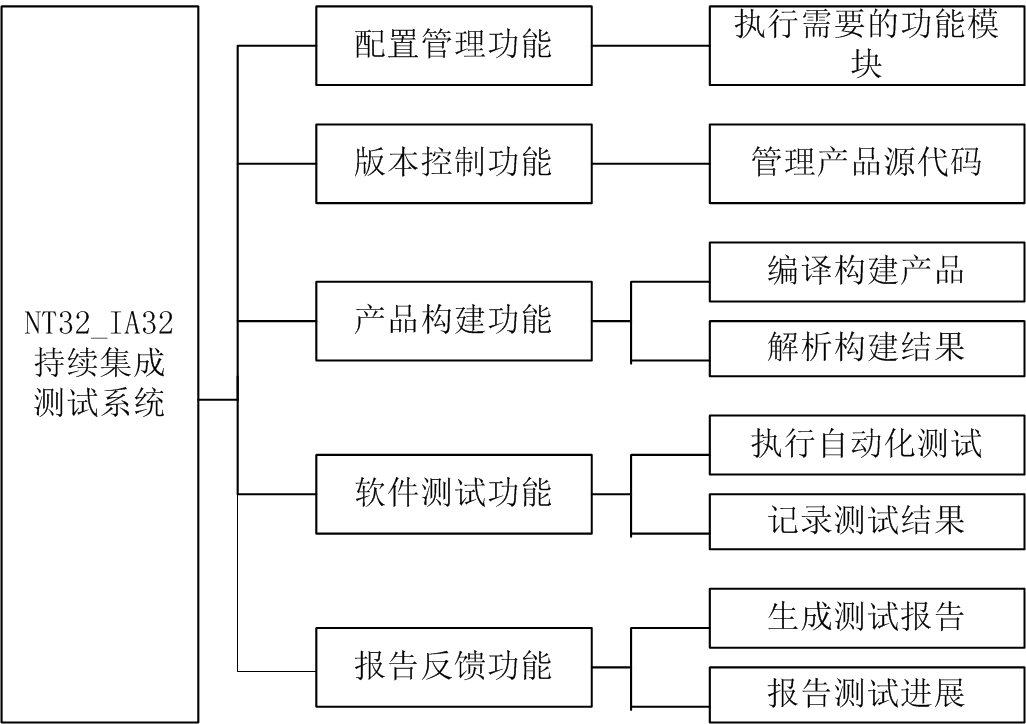
\includegraphics[height=8cm]{chart5/Nt32-IA32持续集成测试系统的功能框架组成}
			\caption{Nt32-IA32持续集成测试系统的功能框架组成}
			\label{fig:Nt32-IA32持续集成测试系统的功能框架组成}
		\end{figure}
		
		其功能框架主要由:1)配置管理功能;2)版本控制功能;3)产品构建功能;4)软件测试功能;5)报告反馈功能五部分模块组成。
	
	\subsection{Nt32-IA32持续集成测试系统的功能流程}
		Nt32-IA32持续集成测试系统的功能流程如图~\ref{fig:Nt32-IA32持续集成测试系统的功能流程}所示:
		
		\begin{figure}[H] % use float package if you want it here
			\centering
			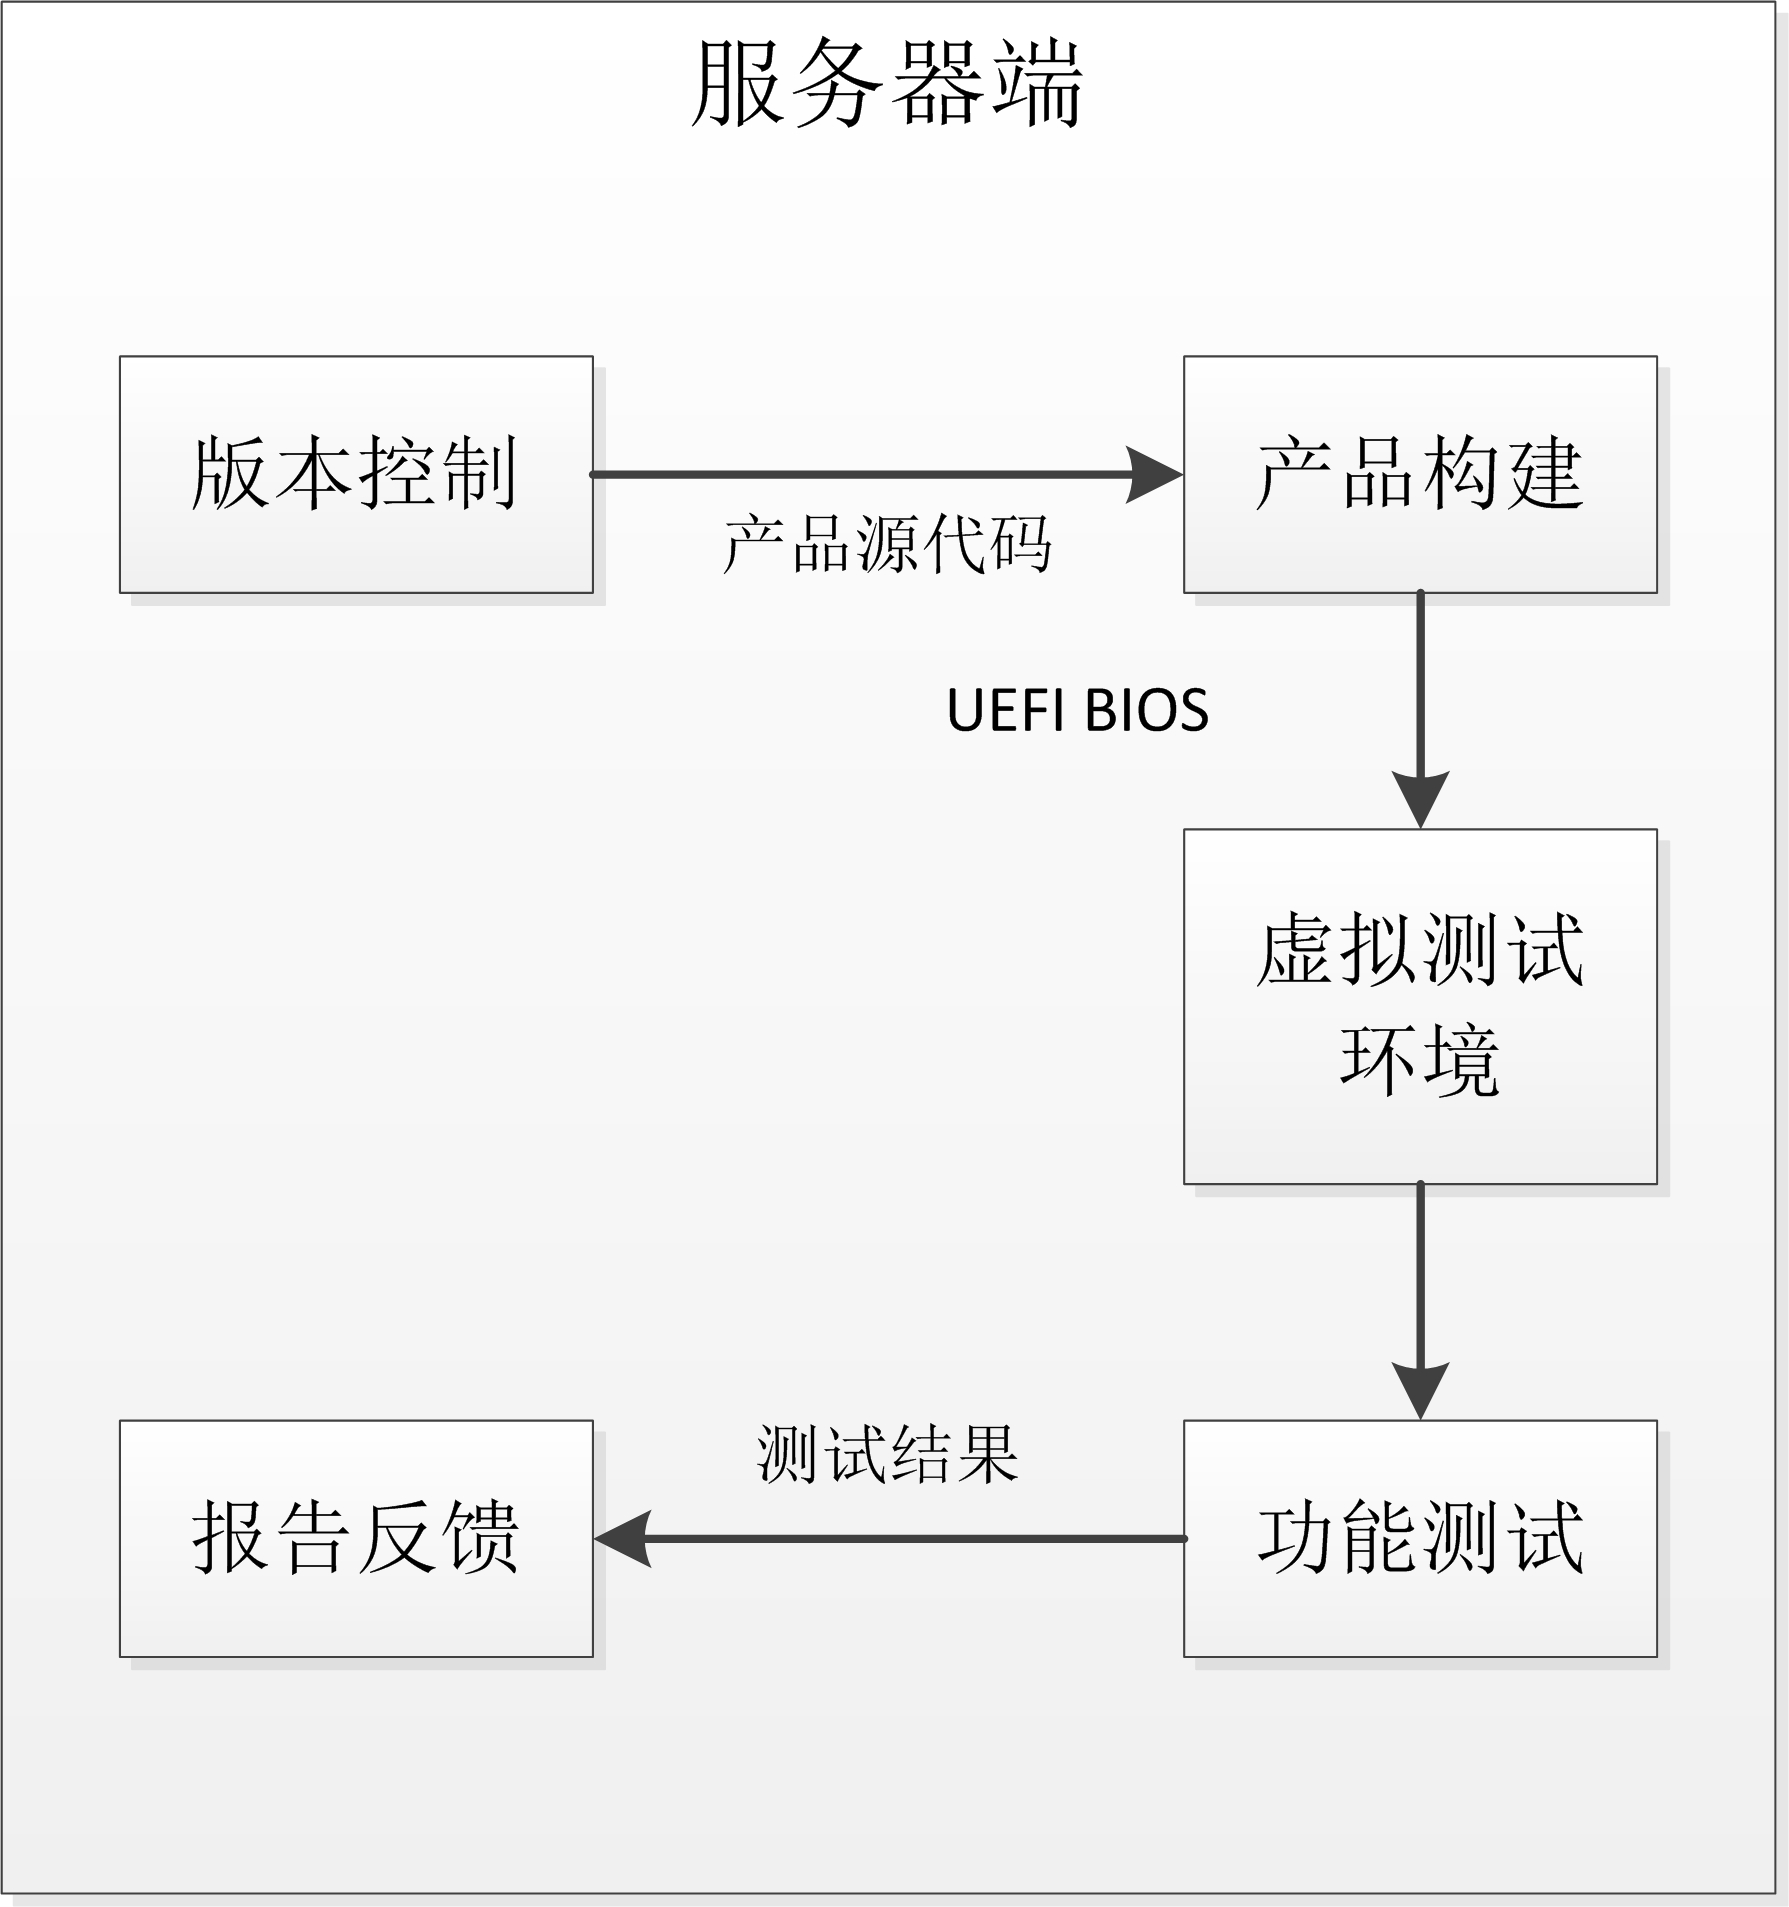
\includegraphics[height=8cm]{chart5/Nt32-IA32持续集成测试系统的功能流程}
			\caption{Nt32-IA32持续集成测试系统的功能流程}
			\label{fig:Nt32-IA32持续集成测试系统的功能流程}
		\end{figure}
		
		服务器负责对整个持续集成测试系统的进行集成调度,其通过版本控制系统从源代码库中获取源文件进行产品构建,在构建好的Nt32模拟器中利用SCT对产品进行功能性测试,并且向相关人员发送产品测试报告。 

\section{Nt32-IA32持续集成测试系统各组成模块的设计与实现}
	
	Nt32-IA32持续集成测试系统主要由配置管理、版本控制、产品构建、软件测试功能和报告反馈五个模块组成。
	
	由于服务器的操作系统为Windows Server 2008,软件测试需要在模拟仿真的UEFI BIOS Shell环境中进行,因此我们最终选用Windows DOS/BAT脚本与UEFI BIOS Shell脚本对该系统进行最终实现。
		
	\subsection{配置管理模块的设计与实现}
		
		为了方便管理Nt32-IA32持续集成测试系统各模块是否执行,因此设计和实现本模块用于对系统进行配置和管理。配置信息对各模块的管理如图~\ref{fig:Nt32-IA32持续集成测试系统配置管理模块的设计与实现}所示:
	
		\begin{figure}[H] % use float package if you want it here
			\centering
			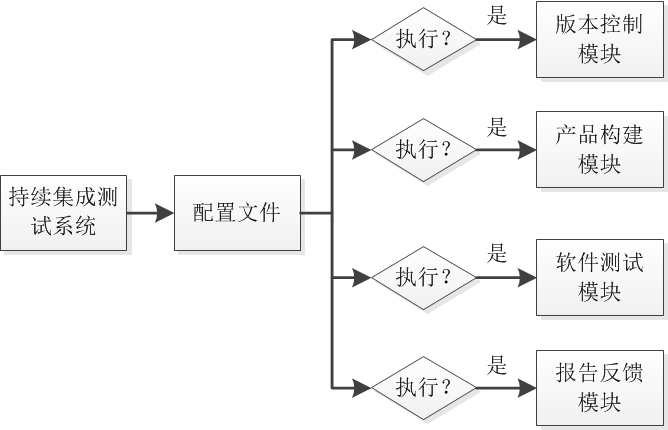
\includegraphics[height=7.5cm]{chart5/Nt32-IA32持续集成测试系统配置管理模块的设计与实现}
			\caption{Nt32-IA32持续集成测试系统配置管理模块的设计与实现}
			\label{fig:Nt32-IA32持续集成测试系统配置管理模块的设计与实现}
		\end{figure}
	
	\subsection{版本控制模块的设计与实现}
		
		版本控制模块的功能流程如图~\ref{fig:Nt32-IA32持续集成测试系统版本控制模块的设计与实现}所示:
		
		\begin{figure}[H] % use float package if you want it here
			\centering
			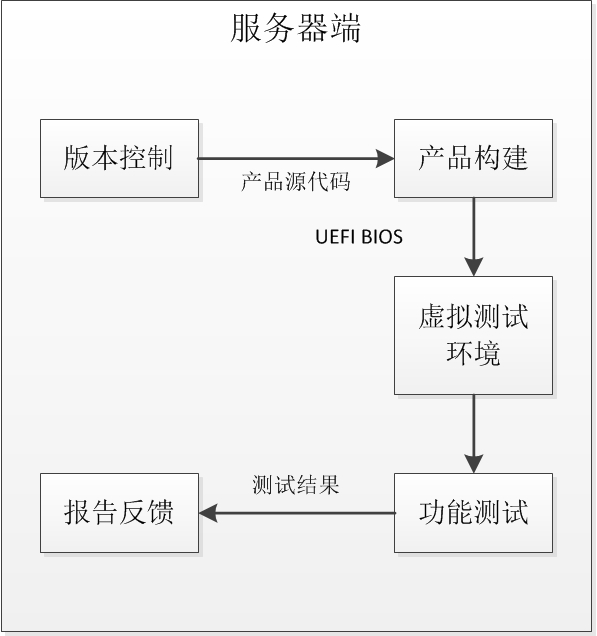
\includegraphics[height=7cm]{chart5/Nt32-IA32持续集成测试系统版本控制模块的设计与实现}
			\caption{Nt32-IA32持续集成测试系统版本控制模块的设计与实现}
			\label{fig:Nt32-IA32持续集成测试系统版本控制模块的设计与实现}
		\end{figure}

		其功能流程与Denlow-X64相同,因此此处不再赘述。
	
	\subsection{产品构建模块的设计与实现}
		
		Nt32-IA32产品构建模块的功能流程如图~\ref{fig:Nt32-IA32持续集成测试系统产品构建模块的设计与实现}所示:
		
		\begin{figure}[H] % use float package if you want it here
			\centering
			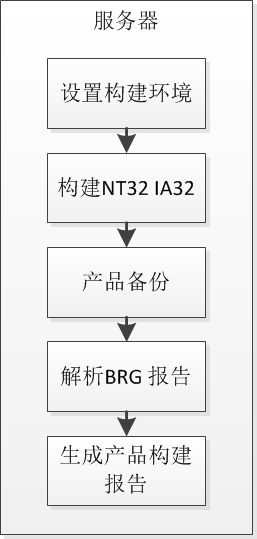
\includegraphics[height=7cm]{chart5/Nt32-IA32持续集成测试系统产品构建模块的设计与实现}
			\caption{Nt32-IA32持续集成测试系统产品构建模块的设计与实现}
			\label{fig:Nt32-IA32持续集成测试系统产品构建模块的设计与实现}
		\end{figure}
		
		其功能流程的设计实现与Denlow-X64大体相同,不同之处大概有以下几点:
		\begin{itemize}
			\item BuildPlatform.bat
			
				BuildPlatform.bat主要用于编译构建产品Nt32-IA32。Build Nt32首先清除掉之前一次的产品构建结果与日志,之后进行产品IA32版本的构建。若有产品出现则判断产品构建成功,将构建的产品进行备份;否则判断产品构建失败。最后将构建过程中产生的报告文件ReportFile.txt进行备份。
			\item GenBuildReport.bat
			
				GenBuildReport.bat主要生成产品构建测试报告。其功能流程如图~\ref{fig:GenNt32BuildReport的功能流程图}所示:
				
				\begin{figure}[H] % use float package if you want it here
					\centering
					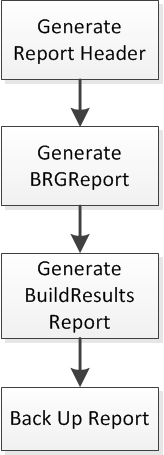
\includegraphics[height=7.5cm]{chart5/GenBuildReport的功能流程图}
					\caption{GenBuildReport的功能流程图}
					\label{fig:GenNt32BuildReport的功能流程图}
				\end{figure}
				
				与Denlow-X64不同的是,Nt32-IA32的产品构建报告不仅包括BRG和产品构建结果,也包括对Shell命令:reconnect -r的测试结果。
		\end{itemize}
	
	\subsection{软件测试模块的设计与实现}
		
		软件测试模块的功能流程如图~\ref{fig:Nt32-IA32持续集成测试系统软件测试模块的设计与实现}所示:
		
		\begin{figure}[H] % use float package if you want it here
			\centering
			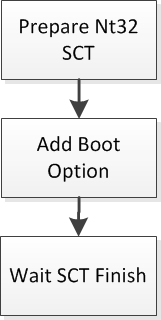
\includegraphics[height=5.5cm]{chart5/Nt32-IA32持续集成测试系统软件测试模块的设计与实现}
			\caption{Nt32-IA32持续集成测试系统软件测试模块的设计与实现}
			\label{fig:Nt32-IA32持续集成测试系统软件测试模块的设计与实现}
		\end{figure}
		
		Prepare Nt32 SCT主要用于部署好用于仿真模拟UEFI BIOS环境的产品,并且将负责控制SCT测试操作的Startup.nsh文件放在产品所在目录。
		
		Add Boot Option主要用于启动构建好的UEFI BIOS模拟器secmain.exe,并且对其进行操作以执行SCT测试。
		
		Wait SCT Finish主要用于监测仿真模拟UEFI BIOS环境下的SCT测试是否完成,测试完成后将测试日志进行备份。
		
	\subsection{报告反馈模块的设计与实现}
		
		报告反馈模块的功能流程如图~\ref{fig:Nt32-IA32持续集成测试系统报告反馈模块的功能流程图}所示:
		
		\begin{figure}[H] % use float package if you want it here
			\centering
			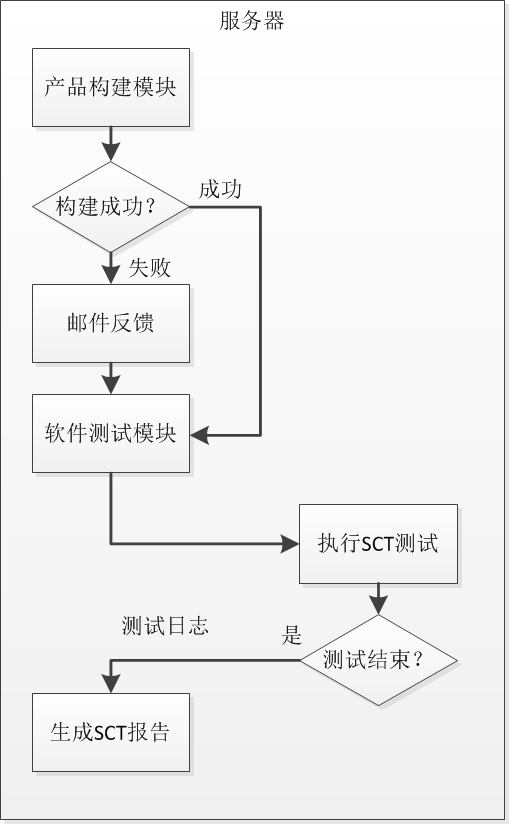
\includegraphics[height=11cm]{chart5/Nt32-IA32持续集成测试系统报告反馈模块的功能流程图}
			\caption{Nt32-IA32持续集成测试系统报告反馈模块的功能流程图}
			\label{fig:Nt32-IA32持续集成测试系统报告反馈模块的功能流程图}
		\end{figure}
		
		其实现方法与Denlow-X64相同,因此不再赘述。
	
	\subsection{系统日志模块的设计与实现}
		
		系统日志模块的设计与Denlow相同,因此不再赘述。如图~\ref{fig:Nt32-IA32持续集成测试系统日志模块的设计与实现}所示:
		
		\begin{figure}[H] % use float package if you want it here
			\centering
			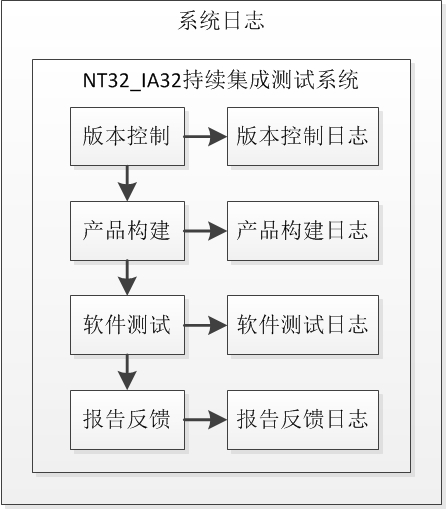
\includegraphics[height=8cm]{chart5/Nt32-IA32持续集成测试系统日志模块的设计与实现}
			\caption{Nt32-IA32持续集成测试系统日志模块的设计与实现}
			\label{fig:Nt32-IA32持续集成测试系统日志模块的设计与实现}
		\end{figure}
		
\section{Nt32-IA32持续集成测试系统运行策略的设计与实现}
	\subsection{Nt32-IA32持续集成测试系统运行策略的设计}
		
		Nt32-IA32持续集成测试系统运行策略的设计与Denlow-X64相同,因此不再赘述。

	\subsection{Nt32-IA32持续集成测试系统运行策略的实现}
		
		与Denlow-X64相似,为了实现这一需求,利用Windows 任务计划能够有效的做到系统的持续性。
		
		main.bat是系统的入口点,利用Windows任务计划定时运行main.bat并且传入参数Nt32,即可启动该系统,自动化的完成该轮持续集成测试的任务。	

\section{Nt32-IA32持续集成测试系统的实验结果}
	\subsection{Nt32-IA32持续集成测试系统的测试报告}
		
		Nt32-IA32持续集成测试系统的报告主要由产品构建报告和产品测试报告两部分组成。
		
		\begin{itemize}
			\item 产品构建报告
			
				产品构建报告负责报告产品构建的情况。以R20406版本的Edk2为例,其产品构建报告的结果如图~\ref{fig:R9Prime-Nt32-Build-Report-Edk2-R20406}所示:
				
				\begin{figure}[H] % use float package if you want it here
					\centering
					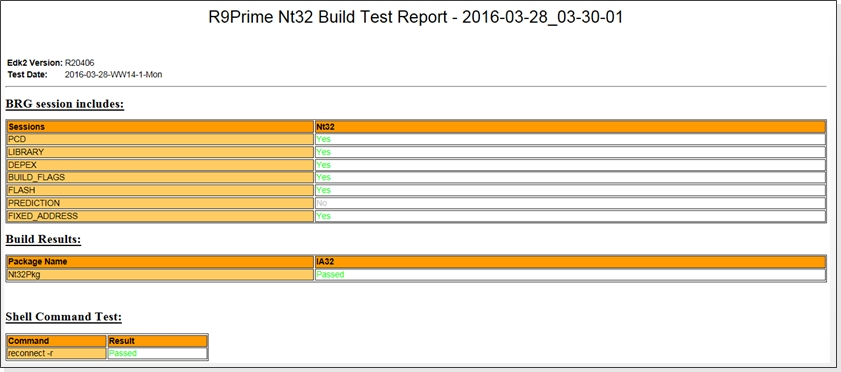
\includegraphics[height=6.8cm]{chart5/R9Prime-Nt32-Build-Report-Edk2-R20406}
					\caption{R9Prime-Nt32-Build-Report-Edk2-R20406}
					\label{fig:R9Prime-Nt32-Build-Report-Edk2-R20406}
				\end{figure}
		
			\item 产品测试报告
			
				产品测试报告主要负责对SCT软件测试的测试结果进行归纳和总结。以R20406版本的Edk2为例,其产品测试报告的结果如图~\ref{fig:R9Prime-Protocol-Test-for-Nt32-Edk2-R20406}所示:
				
				\begin{figure}[H] % use float package if you want it here
					\centering
					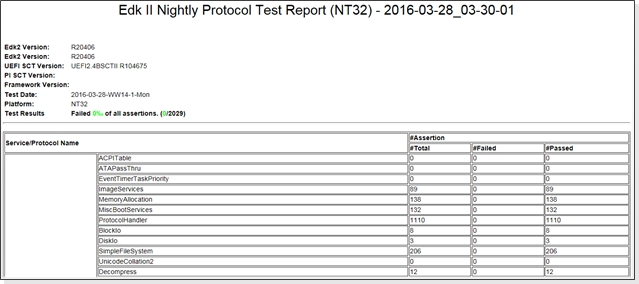
\includegraphics[height=6.8cm]{chart5/R9Prime-Protocol-Test-for-Nt32-Edk2-R20406}
					\caption{R9Prime-Protocol-Test-for-Nt32-Edk2-R20406}
					\label{fig:R9Prime-Protocol-Test-for-Nt32-Edk2-R20406}
				\end{figure}
				
		\end{itemize}
	\subsection{实验结果分析与小结}
		\begin{itemize}
			\item 系统运行时间
			
				以R20406版本的Edk2为例,依据其测试日志文件中的相关信息,该版本下持续集成测试系统的运行时间如表~\ref{tab:Edk2-R20406-Nt32-R20406版本的持续集成测试的运行时间}所示:
				
				\begin{longtable}[c]{c*{3}{r}}
					\caption{Edk2-R20406-Nt32-R20406版本的持续集成测试的运行时间}
					\label{tab:Edk2-R20406-Nt32-R20406版本的持续集成测试的运行时间}\\
					\toprule[1.5pt]
					 测试类型 & \multicolumn{1}{c}{起始时间} & \multicolumn{1}{c}{结束时间} & \multicolumn{1}{c}{耗时} \\\midrule[1pt]
					\endfirsthead
					\multicolumn{4}{c}{续表~\thetable\hskip1em 实验数据}\\
					\toprule[1.5pt]
					 测试类型 & \multicolumn{1}{c}{起始时间} & \multicolumn{1}{c}{结束时间} & \multicolumn{1}{c}{耗时} \\\midrule[1pt]
					\endhead
					\hline
					\multicolumn{4}{r}{续下页}
					\endfoot
					\endlastfoot
					NT32-Build-IA32 & 03:30:01.50 & 03:49:20.47 & 00:19:18.97 \\
					Protocol-Test-for-NT32 & 03:49:20.47 & 05:57:40.60 & 02:08:20.13 \\
					总计 & 03:30:01.50 & 05:57:40.60 & 02:27:39.10 \\
					\bottomrule[1.5pt]
				\end{longtable}
				
				从表中可以看出,Nt32-IA32持续集成测试系统的运行耗时大概在两个半小时左右。由于其较为费时,因此采用每日集成策略,在无人值守的夜晚,自动化运行该系统,以对当前版本的产品进行测试,这样能够大大提高测试的效率,保障项目的高效进行。
			\item 系统运行成功率
			
				以该系统应用到项目开发后,其在一月份、二月份的执行统计为基础,其成功率如表~\ref{tab:Nt32-IA32持续集成测试系统的运行成功率}所示:
				
				\begin{longtable}[c]{c*{3}{r}}
					\caption{Nt32-IA32持续集成测试系统的运行成功率}
					\label{tab:Nt32-IA32持续集成测试系统的运行成功率}\\
					\toprule[1.5pt]
					 月份 & \multicolumn{1}{c}{成功次数} & \multicolumn{1}{c}{失败次数} & \multicolumn{1}{c}{成功率} \\\midrule[1pt]
					\endfirsthead
					\multicolumn{4}{c}{续表~\thetable\hskip1em 实验数据}\\
					\toprule[1.5pt]
					 月份 & \multicolumn{1}{c}{成功次数} & \multicolumn{1}{c}{失败次数} & \multicolumn{1}{c}{成功率} \\\midrule[1pt]
					\endhead
					\hline
					\multicolumn{4}{r}{续下页}
					\endfoot
					\endlastfoot
					1月 & 28 & 2 & 93.3\% \\
					2月 & 27 & 3 & 90.0\% \\
					总计 & 55 & 5 & 91.7\% \\
					\bottomrule[1.5pt]
				\end{longtable}
				
				从表中可以看出,Nt32-IA32持续集成测试系统的运行成功率能够保证在九成以上,这样绝大多数情况下系统均能够正常运行,测试人员只需要在第二天白天对系统测试的结果进行分析和报告即可,能够大大提高测试人员的效率。但是不可避免的仍然有少数情况系统未能够正常运行,其失败原因如表~\ref{tab:一、二月份Nt32-IA32持续集成测试系统运行失败原因分析}所示:
				
				\begin{longtable}[c]{c*{3}{r}}
					\caption{一、二月份Nt32-IA32持续集成测试系统运行失败原因分析}
					\label{tab:一、二月份Nt32-IA32持续集成测试系统运行失败原因分析}\\
					\toprule[1.5pt]
					 系统运行失败原因 & \multicolumn{1}{c}{失败次数} & \multicolumn{1}{c}{失败原因类型} \\\midrule[1pt]
					\endfirsthead
					\multicolumn{4}{c}{续表~\thetable\hskip1em 实验数据}\\
					\toprule[1.5pt]
					 系统运行失败原因 & \multicolumn{1}{c}{失败次数} & \multicolumn{1}{c}{失败原因类型} \\\midrule[1pt]
					\endhead
					\hline
					\multicolumn{4}{r}{续下页}
					\endfoot
					\endlastfoot
					网络问题 &  3  & 系统外部因素  \\
					SVN服务器宕机 &  1  & 系统外部因素  \\
					产品源代码问题 &  1  & 产品质量因素  \\
					\bottomrule[1.5pt]
				\end{longtable}
				
				通过表中对失败原因进行的分析可以看出,系统失败的因素全部为系统外部因素所致。除了网络问题、源代码服务器问题以外,存在着开发过程中对源文件的修改不正确导致产品构建失败的因素,这也正是CI系统能够在第一时间的发现产品集成的问题这一重要意义的体现。
		
		\end{itemize}

\section{本章小结}
    本章主要介绍了Nt32-IA32 持续集成测试系统的设计与实现,并且展示了最终的实验结果并且对其进行了分析和总结。目前该套系统已经成功通过验证,并且部署应用到Nt32-IA32的开发项目中,用于在其敏捷开发的过程中完成每日集成和测试产品的任务。